\documentclass[11pt,a4paper]{article}

\usepackage[utf8]{inputenc}
\usepackage[T1]{fontenc}
\usepackage{lmodern}
\usepackage{geometry}
\usepackage{amsmath, amssymb}
\usepackage{hyperref}
\usepackage{enumitem}
\usepackage{xcolor}
\usepackage{graphicx}

\geometry{margin=2.4cm}
\setlength{\parskip}{0.6em}
\setlength{\parindent}{0pt}

\title{Customer Flow Simulation Through Store Geometry}
\author{}
\date{}

\begin{document}

\maketitle

\begin{abstract}
This idea explores whether customer-flow trajectories inside a store can be used to simulate how visitors would behave under different store-path configurations. The goal is not to predict the exact path of each individual customer, but to estimate the aggregate behaviour of the flow: where visitors concentrate, which areas gain or lose exposure, how congestion changes, and what happens when a shortcut is closed, opened, or redirected.

The analogy comes from statistical mechanics and fluid dynamics. In physics, we do not need to know the precise trajectory of every molecule in a room to describe useful macroscopic properties such as temperature, pressure, or density. Similarly, in a store, we may not be able to predict the exact movement of a single customer, but we can model the collective movement of many customers as a flow through space. Starting from observed trajectories and entry volumes, we can estimate a baseline customer-flow field and then simulate how that flow changes when the store layout is modified.

A first version of the model could use simple deterministic motion equations with added noise, representing customers as particles moving through a store map. The deterministic component would capture the general direction of movement, attraction toward key areas, and resistance created by obstacles or narrow passages. The stochastic component would represent individual variability, hesitation, browsing, shortcuts, and unexpected decisions. In this framework, changes to the store path can be treated like changes in the geometry of a physical system: closing a shortcut, moving an obstacle, or creating a new route changes the flow field and therefore the expected distribution of visitors across the store.

The practical output would be a simulation tool where, given an initial flow of visitors, for example 2,000 daily visitors, we can test scenarios such as: where do customers go under the current layout, what happens if we close a shortcut, which areas receive more or less traffic, and how much additional exposure a new path could generate. This would help evaluate store-path decisions before implementation by estimating their expected impact on customer distribution, area exposure, congestion, and commercial opportunities.
\end{abstract}

\section{Core Idea}

The objective is to model customer movement through a store as a flow through geometry. The model should answer questions such as:

\begin{itemize}[leftmargin=*]
    \item Given 2,000 visitors, where do they go?
    \item What happens if we close a shortcut?
    \item Which areas gain or lose traffic after changing the path?
    \item How does congestion move through the store?
    \item Can a new path increase exposure to under-visited commercial areas?
\end{itemize}

The modelling principle is similar to statistical mechanics: we do not need to predict the exact path of each individual customer. Instead, we aim to predict aggregate quantities such as density, exposure, congestion, and flow distribution.

\section{Store as a Geometry}

Represent the store as a two-dimensional domain:

\begin{equation}
\Omega \subset \mathbb{R}^2
\end{equation}

where:

\begin{itemize}[leftmargin=*]
    \item open walkable space is the valid area of movement;
    \item walls, shelves, displays, and closed shortcuts are obstacles;
    \item entrances and exits define boundary conditions;
    \item departments and commercial areas act as attraction zones;
    \item the main store path defines a preferred direction field.
\end{itemize}

Each customer can then be represented as a moving particle inside this geometry.

\section{Basic Particle Model}

For customer $i$, let the position at time $t$ be:

\begin{equation}
X_i(t) = \bigl(x_i(t), y_i(t)\bigr)
\end{equation}

A simple stochastic motion equation is:

\begin{equation}
\mathrm{d}X_i = v(X_i,t)\,\mathrm{d}t + \sigma\,\mathrm{d}W_t
\end{equation}

where:

\begin{itemize}[leftmargin=*]
    \item $v(X_i,t)$ is the deterministic velocity field;
    \item $\sigma$ controls the level of random movement;
    \item $\mathrm{d}W_t$ is a Brownian noise term representing browsing, hesitation, and individual variability.
\end{itemize}

In business terms:

\begin{quote}
Customer movement = expected store flow + random deviation.
\end{quote}

A discrete-time simulation version is:

\begin{equation}
X_i(t+\Delta t) = X_i(t) + v(X_i,t)\Delta t + \sigma \sqrt{\Delta t}\,\epsilon_i
\end{equation}

with:

\begin{equation}
\epsilon_i \sim \mathcal{N}(0,I)
\end{equation}

This can be used to simulate thousands of visitors and create density maps, heatmaps, and scenario comparisons.

\section{Velocity Field}

The deterministic velocity field can be decomposed into several interpretable components:

\begin{equation}
v(x,t) = v_{\text{path}}(x) + v_{\text{attraction}}(x) + v_{\text{avoidance}}(x) + v_{\text{crowd}}(x,t)
\end{equation}

\subsection{Main Path Force}

The main path force pulls visitors along the intended store route:

\begin{equation}
v_{\text{path}}(x) = \alpha p(x)
\end{equation}

where $p(x)$ is a unit vector pointing along the main path, and $\alpha$ controls the strength of path-following behaviour.

\subsection{Attraction to Areas}

Departments, displays, shortcuts, food areas, or high-interest zones can attract some visitors:

\begin{equation}
v_{\text{attraction}}(x) = \sum_k \beta_k \frac{a_k - x}{\|a_k - x\|}
\end{equation}

where $a_k$ is the location of attraction area $k$, and $\beta_k$ represents its attraction strength.

\subsection{Obstacle Avoidance}

Walls, shelves, closed paths, or bottlenecks repel movement:

\begin{equation}
v_{\text{avoidance}}(x) = - \sum_j \gamma_j \frac{o_j - x}{\|o_j - x\|^2}
\end{equation}

where $o_j$ is the location of obstacle $j$, and $\gamma_j$ controls the repulsion strength.

\subsection{Crowd Pressure}

Visitors tend to avoid highly congested areas. This can be modelled as movement away from high-density regions:

\begin{equation}
v_{\text{crowd}}(x,t) = -\lambda \nabla \rho(x,t)
\end{equation}

where $\rho(x,t)$ is the customer density and $\lambda$ controls sensitivity to congestion.

\section{Fluid or Density Model}

Instead of modelling every individual customer, we can model the aggregate density of customers:

\begin{equation}
\frac{\partial \rho}{\partial t} + \nabla \cdot (\rho v) = D \nabla^2 \rho + S(x,t)
\end{equation}

where:

\begin{itemize}[leftmargin=*]
    \item $\rho(x,t)$ is the density of customers at location $x$ and time $t$;
    \item $v(x,t)$ is the velocity field;
    \item $D\nabla^2\rho$ captures diffusion, random browsing, and dispersion;
    \item $S(x,t)$ is a source term, for example visitor inflow at entrances;
    \item exits can be treated as sinks or absorbing boundaries.
\end{itemize}

This equation is similar to an advection-diffusion model. In business language:

\begin{quote}
Visitors enter the store, follow a preferred flow, diffuse because of browsing behaviour, avoid obstacles, and accumulate in attractive or constrained areas.
\end{quote}

\section{Modelling a Closed Shortcut}

In the continuous geometry model, closing a shortcut means removing that region from the walkable domain:

\begin{equation}
x \notin \Omega
\end{equation}

After simulating the same visitor inflow under the current and proposed layouts, the impact can be measured as:

\begin{equation}
\Delta \rho(x) = \rho_{\text{new}}(x) - \rho_{\text{baseline}}(x)
\end{equation}

For a specific area $A_k$, the change in exposure is:

\begin{equation}
\Delta V_k = \int_{A_k} \Delta \rho(x)\,\mathrm{d}x
\end{equation}

This tells us which areas gain or lose expected traffic.

\section{Simulation Logic}

A simple simulation can follow these steps:

\begin{enumerate}[leftmargin=*]
    \item Start each customer at the entrance.
    \item Assign a profile, such as fast shopper, browser, family visitor, food visitor, or shortcut user.
    \item At each step, choose movement based on path preference, destination attraction, obstacle avoidance, congestion avoidance, and random noise.
    \item Stop the trajectory when the customer exits or reaches checkout.
    \item Aggregate all trajectories into heatmaps, exposure maps, and congestion indicators.
\end{enumerate}

\section{Toy Configuration: First Numerical Integration}

Before applying the method to the full MarketHall geometry, we created a small toy configuration to test whether the particle equation produces interpretable flow patterns. The objective of this experiment is not yet calibration against real customer data. The objective is to verify that the model mechanics are understandable: visitors enter, follow a preferred path, deviate through noise, avoid shelves and walls, react weakly to crowding, and eventually leave through the exit.

The toy store is represented as a small grid with walkable cells, wall or shelf cells, one entrance, one exit, and a shared main path. Two room configurations are compared. The outer boundary, entrance, exit, visitor inflow, and main path are kept fixed. Only the shelf disposition changes. This isolates the effect of changing internal geometry while preserving the same preferred route.

\begin{figure}[htbp]
    \centering
    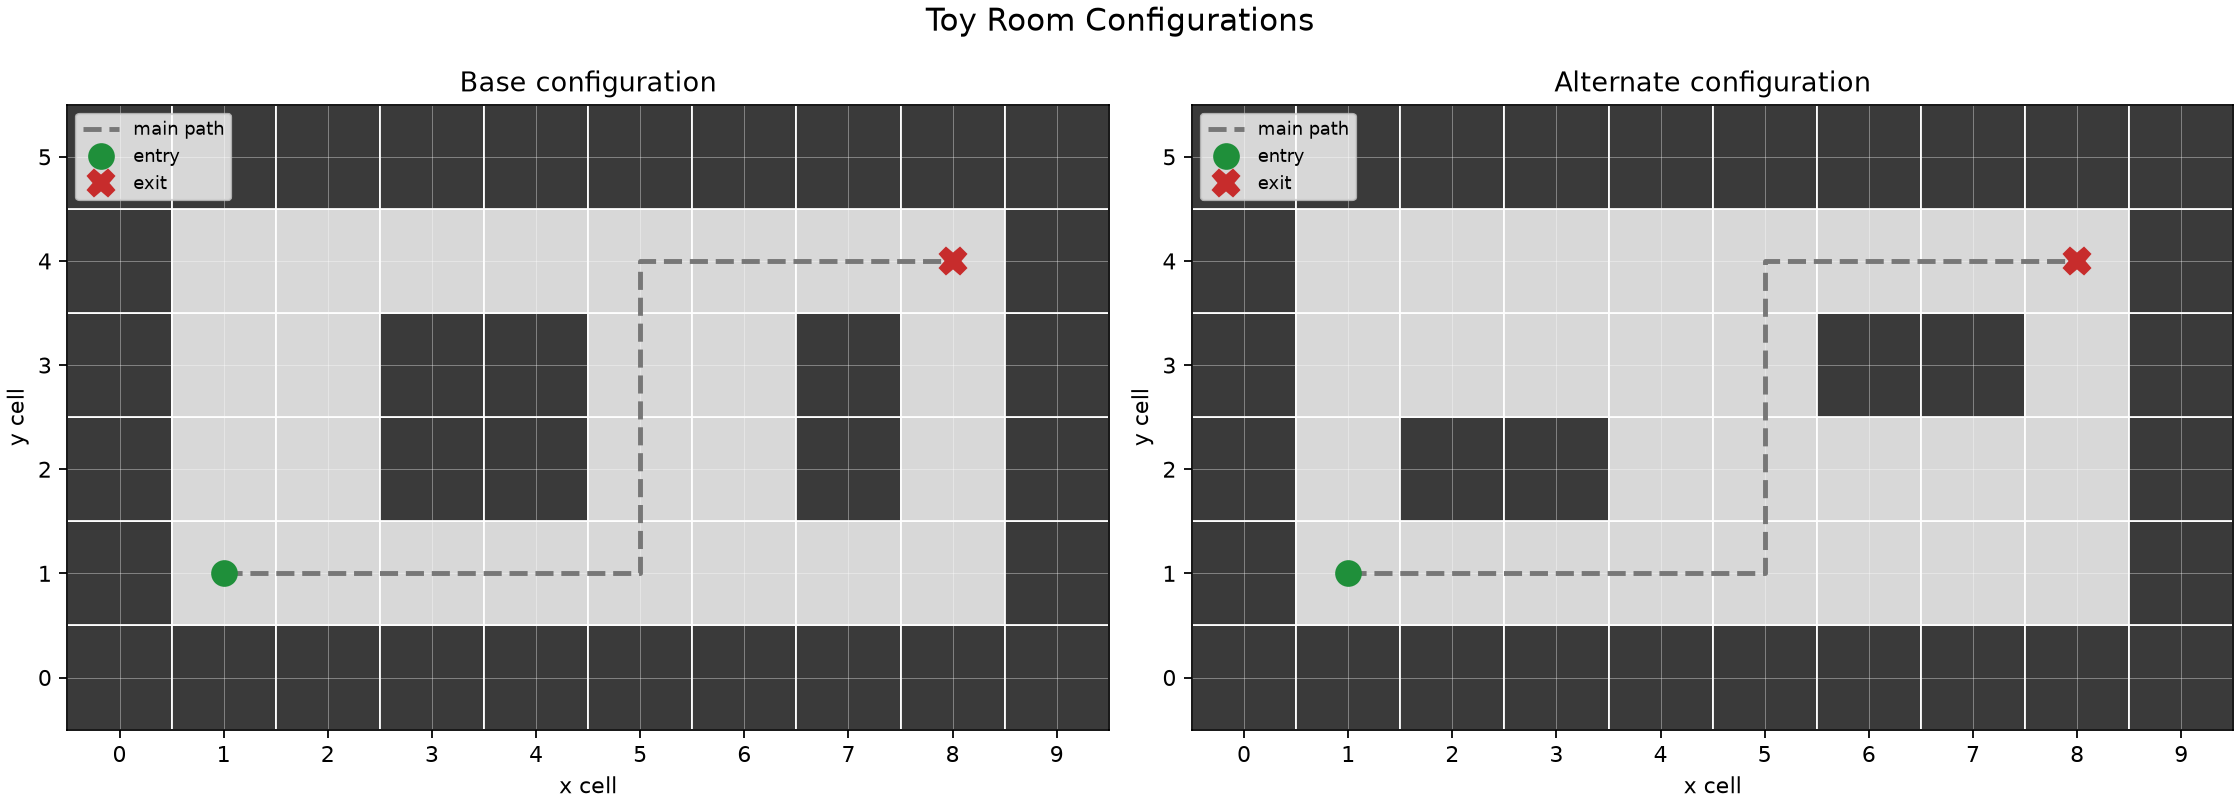
\includegraphics[width=0.95\linewidth]{../toy_configuration/room_configurations.png}
    \caption{Toy room configurations used for the first numerical integration. Both configurations use the same entrance, exit, and main path. The alternate configuration moves one shelf block while keeping the route open.}
    \label{fig:toy-room-configurations}
\end{figure}

For each visitor particle $i$, the simulation integrates the discrete stochastic update:

\begin{equation}
X_i(t+\Delta t) = X_i(t) + v(X_i,t)\Delta t + \sigma \sqrt{\Delta t}\,\epsilon_i,
\qquad \epsilon_i \sim \mathcal{N}(0,I)
\end{equation}

In the toy implementation, the deterministic velocity is:

\begin{equation}
v(x,t) = v_{\text{path}}(x) + v_{\text{avoidance}}(x) + v_{\text{crowd}}(x,t) + v_{\text{wall}}(x)
\end{equation}

The attraction term is disabled in this experiment so that the effect of the geometry is easier to interpret. The current path force has two parts: movement along the route and a distance-scaled correction back toward the nearest point on the route. This avoids the earlier tangent-only behaviour, where particles far from the path could keep moving parallel to the nearest path segment instead of returning toward the route or exit.

The simulated inflow uses 400 particles with a Gaussian arrival profile over time rather than spawning all particles at the beginning. This is closer to a realistic visitor stream: the density at a cell is therefore an accumulated exposure measure over the simulation horizon, not just a final occupancy count.

The main output is a cumulative density heatmap:

\begin{equation}
H(c) = \sum_{t=0}^{T} \sum_i \mathbf{1}\{X_i(t) \in c\}
\end{equation}

where $H(c)$ is the number of particle-time visits to grid cell $c$. In business terms, this is a simple exposure proxy: cells with high values are locations where customers spend more simulated time.

\begin{figure}[htbp]
    \centering
    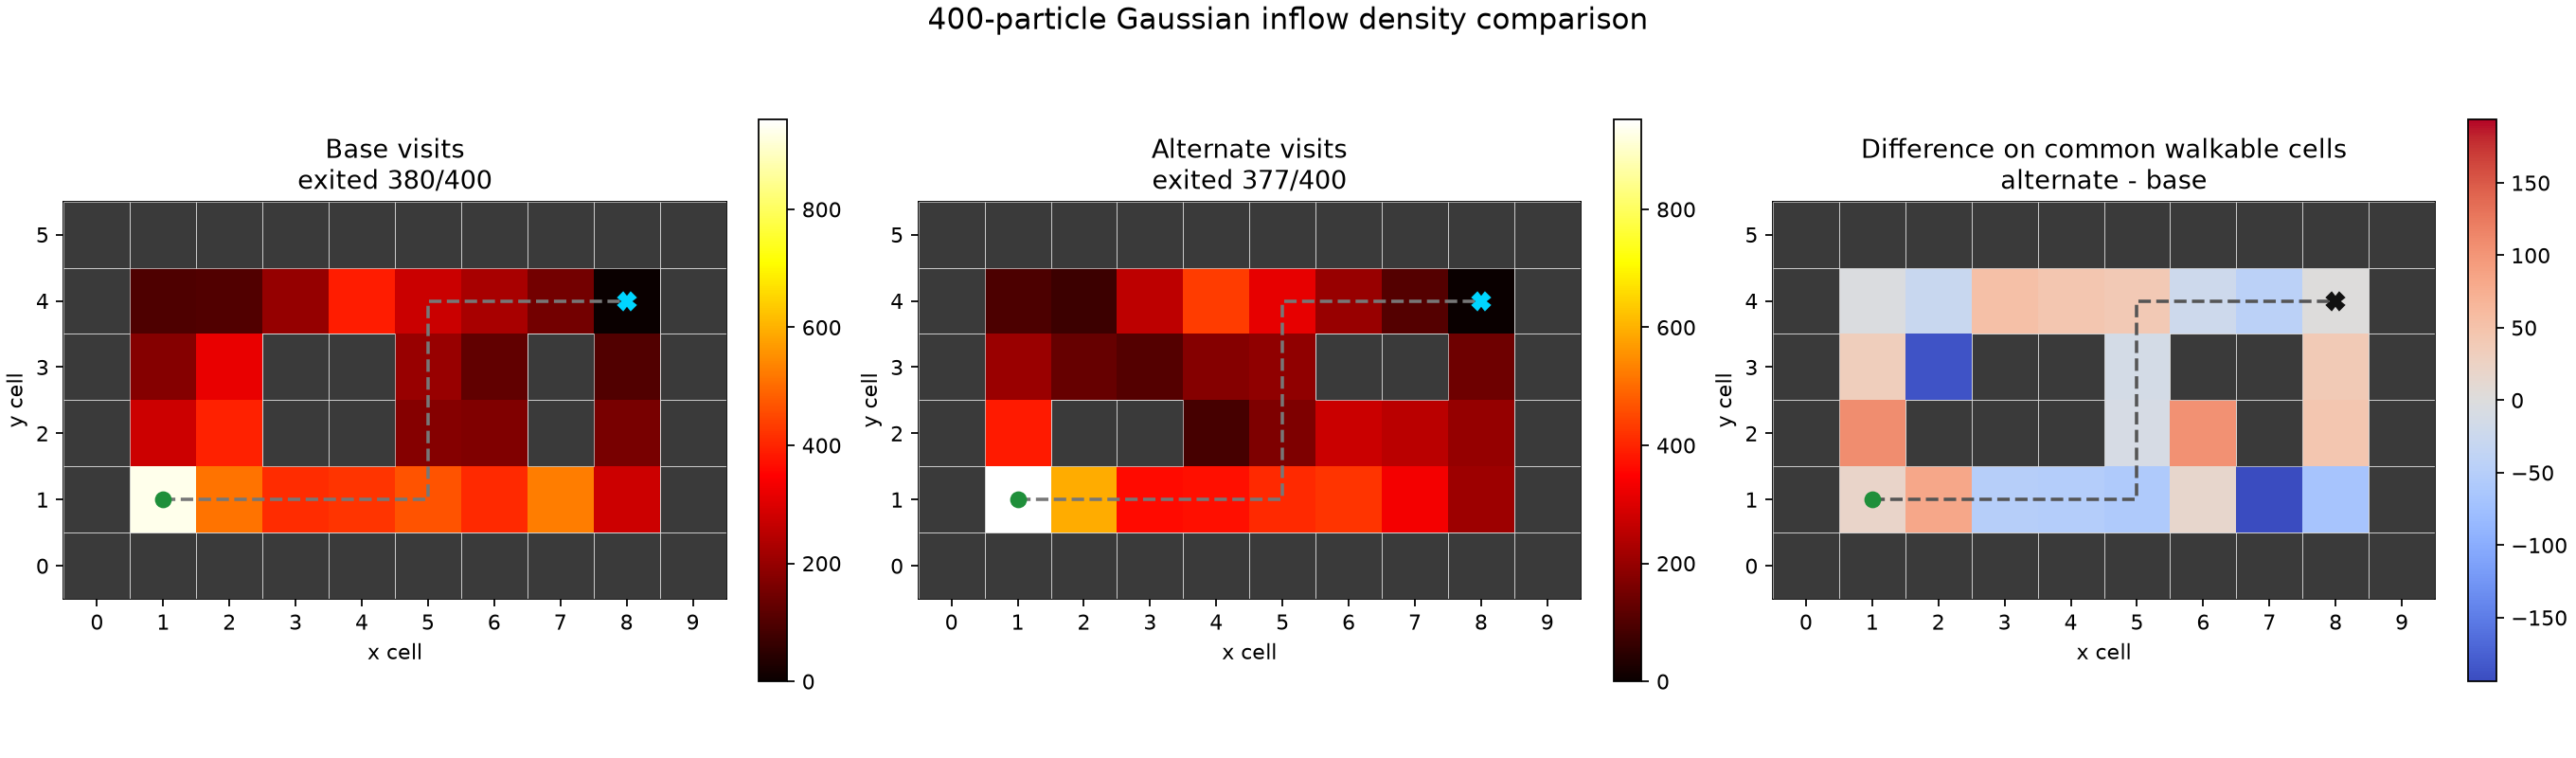
\includegraphics[width=0.95\linewidth]{../toy_configuration/density_heatmap_400p_comparison.png}
    \caption{Preliminary 400-particle density comparison. The first two panels show cumulative visits for the base and alternate configurations. The third panel shows alternate minus base only on cells that are walkable in both layouts, removing trivial differences caused by cells being blocked in one configuration.}
    \label{fig:toy-density-comparison}
\end{figure}

This first result shows what can already be obtained from a simple simulation:

\begin{itemize}[leftmargin=*]
    \item a visual estimate of where customer density accumulates under a given layout;
    \item a like-for-like comparison between two configurations using the same entrance, exit, inflow, main path, and movement parameters;
    \item a difference map showing which shared walkable cells gain or lose exposure after changing shelf placement;
    \item a diagnostic view of whether particles follow the intended path, drift into corners, accumulate near obstacles, or fail to exit within the simulation horizon.
\end{itemize}

In the current 400-particle run, all particles enter the simulation. Most particles exit within the 120-step horizon, while a small number remain active because Gaussian inflow creates late arrivals and random motion can delay some trajectories. This is useful rather than problematic at the prototype stage: it exposes how the choice of simulation horizon, exit radius, path strength, and noise level affects the interpretation of density.

The important point is that the toy model already produces scenario deltas. Once the same logic is transferred to real store geometry and calibrated against observed trajectories, the output can support questions such as: which common walkable areas gain exposure when a shelf is moved, which areas lose traffic, where congestion risk increases, and whether the intended path intervention has the expected directional effect.

\section{Current Prototype Status}

The current prototype has moved from a pure idea into two complementary simulation layers for the Barendrecht MarketHall. These layers are not competing approaches; they answer the same question at different levels of detail.

\subsection{Aggregate Grid Density Simulation}

The first layer is a finite-volume density solver implemented in \texttt{grid\_density\_solver.py}. It uses the MarketHall geometry as a walkable domain and evolves customer density on a grid through an advection-diffusion equation. The current Kompass-based version uses the MarketHall division, walking-path lines, and obstacle geometry from the KMDF file. The model includes:

\begin{itemize}[leftmargin=*]
    \item entry and exit cells;
    \item a main-path velocity field;
    \item diffusion to represent browsing;
    \item attraction toward larger department areas;
    \item a pull back toward the Kompass walking corridor;
    \item removal of customers at exit cells.
\end{itemize}

This is the best layer for aggregate pressure, density, and congestion analysis. It produces time-series density grids, total customers in store over time, and final density maps.

\subsection{Particle Trajectory Simulation}

The second layer is an individual trajectory animation implemented in the grid trajectory animation script. It converts the density model into a particle view: each simulated visitor follows the Kompass corridor, may enter browsing mode, can be attracted by observed heat-grid areas, and is constrained by store obstacles. The current model includes:

\begin{itemize}[leftmargin=*]
    \item corridor-following movement;
    \item random diffusion and stronger browsing diffusion;
    \item heat attraction from observed HFB/grid intensity;
    \item wall and obstacle avoidance;
    \item forced return to the aisle when a particle gets stuck;
    \item simple crowd separation between particles.
\end{itemize}

This is the best layer for communication and qualitative validation, because the animation makes it easy to see whether simulated movement looks plausible inside the real store geometry.

\section{Latest Modelling Idea}

The latest direction is to use the Kompass geometry as the physical constraint and Ariadne observations as calibration signals. In practice, the model should separate two tasks:

\begin{enumerate}[leftmargin=*]
    \item Preserve the store physics: visitors must remain inside walkable MarketHall geometry, follow plausible corridors, avoid walls and shelves, and eventually leave through exit regions.
    \item Calibrate commercial behaviour: observed trajectories, heat grids, dwell patterns, and HFB exposure shares should tune attraction, browsing probability, speed, diffusion, and congestion sensitivity.
\end{enumerate}

The proposed modelling stack is therefore:

\begin{quote}
Kompass geometry defines where customers can move; Ariadne data estimates how customers tend to move; scenario parameters define what changes in the layout or path strategy.
\end{quote}

The short-term goal is not to create a perfect digital twin. The goal is to create a scenario simulator that can answer directional business questions before making a physical store change:

\begin{itemize}[leftmargin=*]
    \item If a shortcut is closed, which areas lose exposure and which areas gain exposure?
    \item If the main path is made stronger, does traffic become more concentrated or more evenly distributed?
    \item If a high-interest area is moved or promoted, how does browsing density shift?
    \item Which path changes create congestion risk near obstacles, corners, or narrow corridors?
\end{itemize}

The most useful next validation step is to compare simulated exposure against observed Ariadne exposure at HFB or grid-cell level, then tune the model parameters until the baseline simulation reproduces the observed distribution closely enough. Once the baseline is credible, scenario deltas become the main decision output.

The basic update equation is:

\begin{equation}
X_i(t+\Delta t) = X_i(t) + v(X_i,t)\Delta t + \sigma \sqrt{\Delta t}\,\epsilon_i
\end{equation}

\section{Calibration with Real Data}

Observed trajectory data can be used to estimate the model parameters:

\begin{itemize}[leftmargin=*]
    \item entry flow by time of day;
    \item average speed;
    \item dwell time by area;
    \item probability of entering each department;
    \item shortcut usage;
    \item congestion sensitivity;
    \item attraction strength of specific zones.
\end{itemize}

A simple calibration objective is:

\begin{equation}
\min_{\theta} \sum_x \left( \rho_{\text{observed}}(x) - \rho_{\text{simulated}}(x;\theta) \right)^2
\end{equation}

where $\theta$ contains parameters such as attraction, friction, noise, walking speed, and congestion sensitivity.

\section{Business KPIs from the Model}

\subsection{Exposure per Area}

\begin{equation}
E_k = \int_0^T \int_{A_k} \rho(x,t)\,\mathrm{d}x\,\mathrm{d}t
\end{equation}

\subsection{Change in Exposure}

\begin{equation}
\Delta E_k = E_k^{\text{new path}} - E_k^{\text{current path}}
\end{equation}

\subsection{Congestion}

One possible congestion metric is maximum density:

\begin{equation}
G_k = \max_t \rho_k(t)
\end{equation}

Another option is time spent above a congestion threshold:

\begin{equation}
G_k = \int_0^T \mathbf{1}_{\rho_k(t)>\rho^*}\,\mathrm{d}t
\end{equation}

\subsection{Commercial Potential}

A simplified link between exposure and sales can be written as:

\begin{equation}
\Delta \text{Sales}_k \approx \Delta E_k \times CR_k \times AOV_k
\end{equation}

where:

\begin{itemize}[leftmargin=*]
    \item $CR_k$ is the conversion rate for area $k$;
    \item $AOV_k$ is the average order value or basket contribution;
    \item $\Delta E_k$ is the change in customer exposure.
\end{itemize}

\section{Recommended Modelling Roadmap}

\subsection*{Phase 1: Grid Density Simulation}

The first practical version should use the Kompass MarketHall geometry as the walkable domain and solve aggregate customer density on a grid.

\begin{quote}
Given a visitor inflow, where does density accumulate if we close, open, or redirect path X?
\end{quote}

For the first Barendrecht MarketHall configuration, the model should use the MarketHall polygon, walking-path corridor, entry and exit cells, and obstacle geometry. The first output is not individual path prediction, but an aggregate exposure and density estimate:

\begin{equation}
E_k = \int_0^T \int_{A_k} \rho(x,t)\,\mathrm{d}x\,\mathrm{d}t
\end{equation}

This can be compared directly with observed Ariadne exposure by HFB or grid cell as a first calibration check.

\subsection*{Phase 2: Particle Simulation}

More visual and intuitive. Generates simulated trajectories and heatmaps.

\begin{quote}
Customers are represented as particles moving through store geometry with noise.
\end{quote}

\subsection*{Phase 3: Calibration with Real Trajectories}

Use observed tracking data to estimate parameters and validate predictions before applying the model to new scenarios.

\section{Positioning Sentence}

\begin{quote}
We cannot predict the exact path of each customer, just as statistical mechanics does not predict the exact path of each molecule. But by modelling customer trajectories as a noisy flow through store geometry, we can estimate the overall impact of path changes on traffic, exposure, and congestion across the store.
\end{quote}

\end{document}
